% slide 15: overview of features. Include list of feature names and highlight ones to describe in detail next.
\begin{frame}
  \frametitle{Features}
    \begin{itemize}
     \item Link properties
      \begin{itemize}
       \item position
       \item order
       \item count
       \item symmetric linking
      \end{itemize}
      
      \item Popularity 
      \begin{itemize}
       \item popularity of resource 
       \item popularity of percentile rank
      \end{itemize}
      
      \item Articles similarity
      \begin{itemize}
       \item link relatedness
       \item text similarity
       \item title similarity
      \end{itemize}

   \item Community membership
   \item Hits and PageRank

  \end{itemize}
\end{frame}


% slide 16: simple link feature introduction: link order
\begin{frame}
  \frametitle{Link order}
      \begin{figure}[h]
   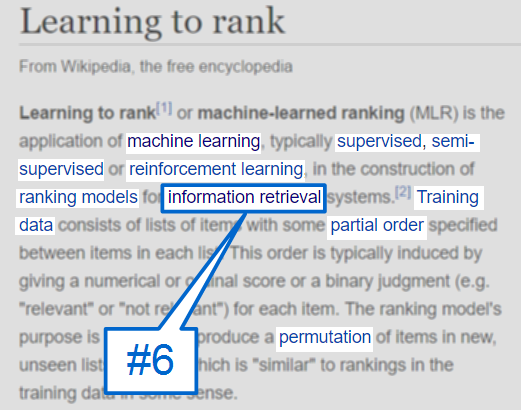
\includegraphics[height=0.6\textheight]{images/link_order}
  \end{figure}
  \begin{itemize}
    \item Motivation:
    \begin{itemize}
     \item Readers habit to read first paragraphs
     \item Main concepts in the leading section
	\end{itemize}
    \item Extracted from Wikipedia dumps
  \end{itemize}
\end{frame}

% slide 17: link symmetry
\begin{frame}
  \frametitle{Symmetrical linking}
  
  \begin{figure}[h]
   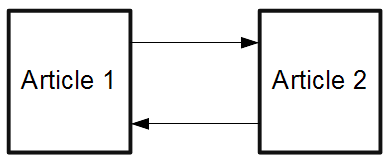
\includegraphics[width=0.75\textwidth]{images/symmetry}
  \end{figure}
  
   \begin{itemize}
   \item Binary feature
   \item Motivation: Highly related topics 
   \item Extracted from Wikipedia dumps
   \end{itemize}

\end{frame}

% slide 18: Motivaltion for similarity features
% slide 19: "Text similarity" feature
\begin{frame}
  \frametitle{Similarity features}
  Measuring relatedness of two linked articles  
\begin{itemize}
\item Text
\item Links
\item Title
\end{itemize}
\textbf{Motivation}: users are more likely to switch to a related topic  
\end{frame}

\begin{frame}
  \frametitle{Example: "Text similarity"}
  \begin{itemize}
\item Measure semantic similarity between two articles 
\item Extract text from Wikipedia dumps
\end{itemize}

    \begin{figure}[h]
    \centering
   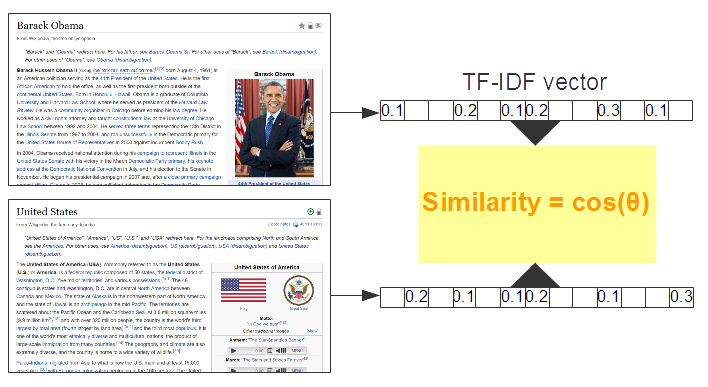
\includegraphics[height=0.75\textheight]{images/similarity}
  \end{figure}
\end{frame}

% slide 20: Motivation for community features
% slide 21: "Community 3" feature
\begin{frame}
   \frametitle{Community features}
\begin{itemize}
\item Graph representation
\item \textbf{Communities}: clusters of interconnected articles
\end{itemize}
\textbf{Motivation}: Two articles of the same community should discuss a similar topic

  \begin{figure}[h]
   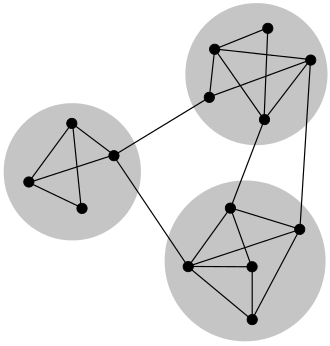
\includegraphics[height=0.4\textheight]{images/communities}
   \caption{Sketch of a small network displaying community structure}
  \end{figure}
 
\end{frame}

\begin{frame}
   \frametitle{Example: "Community 3"}
   \begin{itemize}
\item Extract links from Wikipedia dumps
\item Build the graph
\begin{itemize}
\item Vertices: articles
\item Edges: links
\end{itemize}
\item Distinguish communities with InfoMAP algorithm
\end{itemize}
Binary feature: 1 if both articles belongs to the same community, 0 otherwise
\end{frame}

% slide 22: Motivation for Interest features
% slide 23: "Search Interest" feature
\begin{frame}
   \frametitle{Interest features}
   \textbf{Interest}: number of page views

   \begin{itemize} 
   \item Extracted from Clickstream data
   
   \begin{itemize}
\item External traffic from Google, Yahoo and Bing
\item External traffic from Facebook and Twitter

\end{itemize}
\item Does not depend on current article
\end{itemize}
   \textbf{Motivation}: Readers may have a tendency to follow links to articles on trending and popular topics.
   
\end{frame}

\begin{frame}
   \frametitle{Example: "Search Interest"}
     \begin{figure}[h]
   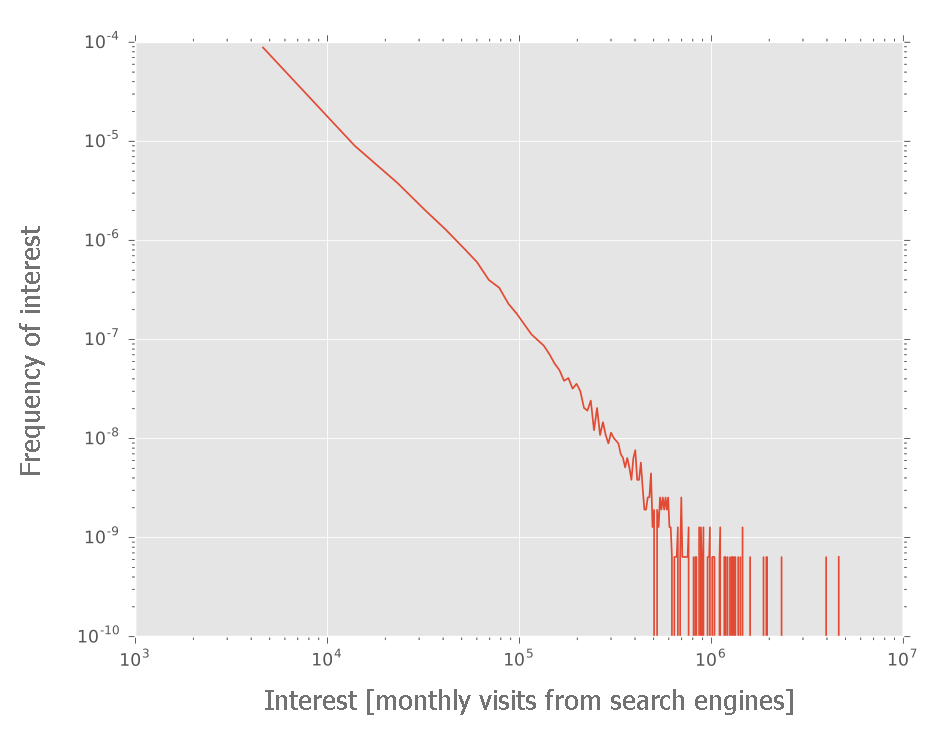
\includegraphics[height=0.6\textheight]{images/pwl_graph}
  \end{figure}
   
   \begin{itemize}
\item Search traffic assumed driven by social networks
\item Social networks form scale-free graphs
\item Interest follows a power law distribution
\item Feature defined by logarithm of search interest
\end{itemize}
   
\end{frame}